
\documentclass[../_main/handlingar.tex]{subfiles}

\begin{document}
\motion{StraffBong}
Styrelsen samt SRE-Ordförande har inte varit så bra på att lägga ut protokoll det senaste året och
enligt Stadgan \S13:2 ska protokollet vara klarjusterad efter åtta (8) läsdagar och enligt §13:3 ska de
finnas tillgängliga på sektionens anslagstavlor och webbplats efter justeringen. Detta har då inte
skett (se bildbevis under). Detta är oacceptabelt och därför anser jag att för varje dag protokollet är
försenat ska Ordförande samt justeringspersonen eller SRE-Ordförande ta en straffbong av en
godtycklig alkoholhaltig dryck.

\begin{center}
  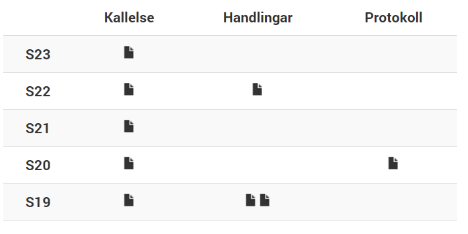
\includegraphics{../_res/protokoll.png}
\end{center}

Därför yrkar jag på

\begin{attsatser}
\att Ordförande, Justeringsperson eller annan ansvarig tar en straffbong för varje dag protokollet är
försenad
\att i stadgan under \S13:3 ändra till:\par
I \S13:1 och \S13:2 nämnda protokoll skall sedan de justerats finnas
tillgängliga på sektionens anslagstavla och webbplats \hl{och varje läsdag försenad straffas med en straffbong}.

\changenote
\end{attsatser}
\begin{signatures}{1}
    Signerat
    \signature{Godtycklig Sektionsmedlem}{Bongare}
\end{signatures}

\end{document}
